\documentclass{ximera}
%\usepackage{todonotes}

\newcommand{\todo}{}

\usepackage{tkz-euclide}
\tikzset{>=stealth} %% cool arrow head
\tikzset{shorten <>/.style={ shorten >=#1, shorten <=#1 } } %% allows shorter vectors

\usepackage{tkz-tab}  %% sign charts
\usetikzlibrary{decorations.pathreplacing} 

\usetikzlibrary{backgrounds} %% for boxes around graphs
\usetikzlibrary{shapes,positioning}  %% Clouds and stars
\usetikzlibrary{matrix} %% for matrix
\usepgfplotslibrary{polar} %% for polar plots
\usetkzobj{all}
\usepackage[makeroom]{cancel} %% for strike outs
%\usepackage{mathtools} %% for pretty underbrace % Breaks Ximera
\usepackage{multicol}

\usepackage{polynom}



\usepackage[many]{tcolorbox}  %% for titled boxes
\newtcolorbox{xbox}[1]{%
    tikznode boxed title,
    enhanced,
    arc=0mm,
    interior style={white},
    attach boxed title to top center= {yshift=-\tcboxedtitleheight/2},
    fonttitle=\bfseries,
    colbacktitle=white,coltitle=black,
    boxed title style={size=normal,colframe=white,boxrule=0pt},
    title={#1}}


\usepackage{array}
\setlength{\extrarowheight}{+.1cm}   
\newdimen\digitwidth
\settowidth\digitwidth{9}
\def\divrule#1#2{
\noalign{\moveright#1\digitwidth
\vbox{\hrule width#2\digitwidth}}}





\newcommand{\RR}{\mathbb R}
\newcommand{\R}{\mathbb R}
\newcommand{\N}{\mathbb N}
\newcommand{\Z}{\mathbb Z}

%\renewcommand{\d}{\,d\!}
\renewcommand{\d}{\mathop{}\!d}
\newcommand{\dd}[2][]{\frac{\d #1}{\d #2}}
\newcommand{\pp}[2][]{\frac{\partial #1}{\partial #2}}
\renewcommand{\l}{\ell}
\newcommand{\ddx}{\frac{d}{\d x}}
\newcommand{\ddt}{\frac{d}{\d t}}

\newcommand{\zeroOverZero}{\ensuremath{\boldsymbol{\tfrac{0}{0}}}}
\newcommand{\inftyOverInfty}{\ensuremath{\boldsymbol{\tfrac{\infty}{\infty}}}}
\newcommand{\zeroOverInfty}{\ensuremath{\boldsymbol{\tfrac{0}{\infty}}}}
\newcommand{\zeroTimesInfty}{\ensuremath{\small\boldsymbol{0\cdot \infty}}}
\newcommand{\inftyMinusInfty}{\ensuremath{\small\boldsymbol{\infty - \infty}}}
\newcommand{\oneToInfty}{\ensuremath{\boldsymbol{1^\infty}}}
\newcommand{\zeroToZero}{\ensuremath{\boldsymbol{0^0}}}
\newcommand{\inftyToZero}{\ensuremath{\boldsymbol{\infty^0}}}



\newcommand{\numOverZero}{\ensuremath{\boldsymbol{\tfrac{\#}{0}}}}
\newcommand{\dfn}{\textbf}
%\newcommand{\unit}{\,\mathrm}
\newcommand{\unit}{\mathop{}\!\mathrm}
\newcommand{\eval}[1]{\bigg[ #1 \bigg]}
\newcommand{\seq}[1]{\left( #1 \right)}
\renewcommand{\epsilon}{\varepsilon}
\renewcommand{\iff}{\Leftrightarrow}

\DeclareMathOperator{\arccot}{arccot}
\DeclareMathOperator{\arcsec}{arcsec}
\DeclareMathOperator{\arccsc}{arccsc}
\DeclareMathOperator{\si}{Si}
\DeclareMathOperator{\proj}{proj}
\DeclareMathOperator{\scal}{scal}


\newcommand{\tightoverset}[2]{% for arrow vec
  \mathop{#2}\limits^{\vbox to -.5ex{\kern-0.75ex\hbox{$#1$}\vss}}}
\newcommand{\arrowvec}[1]{\tightoverset{\scriptstyle\rightharpoonup}{#1}}
\renewcommand{\vec}{\mathbf}
\newcommand{\veci}{\vec{i}}
\newcommand{\vecj}{\vec{j}}
\newcommand{\veck}{\vec{k}}
\newcommand{\vecl}{\boldsymbol{\l}}

\newcommand{\dotp}{\bullet}
\newcommand{\cross}{\boldsymbol\times}
\newcommand{\grad}{\boldsymbol\nabla}
\newcommand{\divergence}{\grad\dotp}
\newcommand{\curl}{\grad\cross}
%\DeclareMathOperator{\divergence}{divergence}
%\DeclareMathOperator{\curl}[1]{\grad\cross #1}


\colorlet{textColor}{black} 
\colorlet{background}{white}
\colorlet{penColor}{blue!50!black} % Color of a curve in a plot
\colorlet{penColor2}{red!50!black}% Color of a curve in a plot
\colorlet{penColor3}{red!50!blue} % Color of a curve in a plot
\colorlet{penColor4}{green!50!black} % Color of a curve in a plot
\colorlet{penColor5}{orange!80!black} % Color of a curve in a plot
\colorlet{fill1}{penColor!20} % Color of fill in a plot
\colorlet{fill2}{penColor2!20} % Color of fill in a plot
\colorlet{fillp}{fill1} % Color of positive area
\colorlet{filln}{penColor2!20} % Color of negative area
\colorlet{fill3}{penColor3!20} % Fill
\colorlet{fill4}{penColor4!20} % Fill
\colorlet{fill5}{penColor5!20} % Fill
\colorlet{gridColor}{gray!50} % Color of grid in a plot

\newcommand{\surfaceColor}{violet}
\newcommand{\surfaceColorTwo}{redyellow}
\newcommand{\sliceColor}{greenyellow}




\pgfmathdeclarefunction{gauss}{2}{% gives gaussian
  \pgfmathparse{1/(#2*sqrt(2*pi))*exp(-((x-#1)^2)/(2*#2^2))}%
}


%%%%%%%%%%%%%
%% Vectors
%%%%%%%%%%%%%

%% Simple horiz vectors
\renewcommand{\vector}[1]{\left\langle #1\right\rangle}


%% %% Complex Horiz Vectors with angle brackets
%% \makeatletter
%% \renewcommand{\vector}[2][ , ]{\left\langle%
%%   \def\nextitem{\def\nextitem{#1}}%
%%   \@for \el:=#2\do{\nextitem\el}\right\rangle%
%% }
%% \makeatother

%% %% Vertical Vectors
%% \def\vector#1{\begin{bmatrix}\vecListA#1,,\end{bmatrix}}
%% \def\vecListA#1,{\if,#1,\else #1\cr \expandafter \vecListA \fi}

%%%%%%%%%%%%%
%% End of vectors
%%%%%%%%%%%%%

%\newcommand{\fullwidth}{}
%\newcommand{\normalwidth}{}



%% makes a snazzy t-chart for evaluating functions
%\newenvironment{tchart}{\rowcolors{2}{}{background!90!textColor}\array}{\endarray}

%%This is to help with formatting on future title pages.
\newenvironment{sectionOutcomes}{}{} 



%% Flowchart stuff
%\tikzstyle{startstop} = [rectangle, rounded corners, minimum width=3cm, minimum height=1cm,text centered, draw=black]
%\tikzstyle{question} = [rectangle, minimum width=3cm, minimum height=1cm, text centered, draw=black]
%\tikzstyle{decision} = [trapezium, trapezium left angle=70, trapezium right angle=110, minimum width=3cm, minimum height=1cm, text centered, draw=black]
%\tikzstyle{question} = [rectangle, rounded corners, minimum width=3cm, minimum height=1cm,text centered, draw=black]
%\tikzstyle{process} = [rectangle, minimum width=3cm, minimum height=1cm, text centered, draw=black]
%\tikzstyle{decision} = [trapezium, trapezium left angle=70, trapezium right angle=110, minimum width=3cm, minimum height=1cm, text centered, draw=black]

\author{Bart Snapp\and Nela Lakos}
\license{Creative Commons 3.0 By-NC}
\acknowledgement{https://www.whitman.edu/mathematics/calculus/}
  \outcome{Interpret an optimization problem as the procedure used to make a system or design as effective or functional as possible.}
  \outcome{Set up an optimization problem by identifying the objective function and appropriate constraints.}
  \outcome{Solve optimization problems by finding the appropriate absolute extremum.}
  \outcome{Solve basic word problems involving maxima or minima.}
\begin{document}
\begin{exercise}

  
  A box with square base and no top is to hold a volume $100$.  Find
  the dimensions of the box that requires the least material for the
  five sides.
  \begin{hint}
  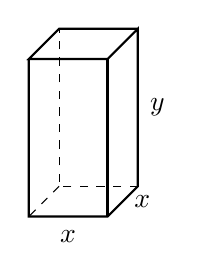
\begin{tikzpicture}

\pgfmathsetmacro{\xr}{2}
\pgfmathsetmacro{\xl}{1}
\pgfmathsetmacro{\yt}{0}
\pgfmathsetmacro{\yb}{-2}
\pgfmathsetmacro{\zi}{0}
\pgfmathsetmacro{\zo}{1}
  \draw[thick](\xr,\yt,0)--(\xl,\yt,\zi)--(\xl,\yt,\zo)--(\xr,\yt,\zo)--(\xr,\yt,\zi)--(\xr,\yb,\zi)--(\xr,\yb,\zo)--(\xl,\yb,\zo)--(\xl,\yt,\zo);
  \draw[thick](\xr,\yt,\zo)--(\xr,\yb,\zo);
  \draw[dashed](\xr,\yb,\zi)--(\xl,\yb,\zi)--(\xl,\yt,\zi);
  \draw[dashed](\xl,\yb,\zi)--(\xl,\yb,\zo);
  \draw(\xr+.25,\yt*.5+\yb*.5,\zi) node{$y$};
  \draw(\xr+.25,\yb,\zi*.5+\zo*.5) node{$x$};
  \draw(\xl*.5+\xr*.5,\yb-.25,\zo) node{$x$};

  \end{tikzpicture}
  \end{hint}
  \begin{hint}
  The dimensions that will result in  "least material" for the five sides are dimensions that result in "smallest surface area".
  So, the quantity that we have to "minimize" is the surface area, $S$.
  \end{hint}
  \begin{hint}
  We have to "minimize"  the surface area, $S$.
  
  $S=x^2 +4xy$
  
  Remember, no top!
  \end{hint}
    \begin{hint}
Next, we express $S$ as a function of, say, $x$.
In order to do that, we have to express $y$ in terms of $x$.


We know that  $V=100$. Therefore,

$x^2\cdot \answer{ y}=100$,
and 

$y=\frac{100}{\answer{x^2}}$.
  
 It follows that 
  
   $S(x)=x^2 +\frac{400}{\answer{x}}$.

  \end{hint}
  \begin{hint}
  So, we have to find the (global) minimum of $S$ on its domain, $(0,\answer{\infty})$.
  We have to find critical points of $S$.
  Therefore, we have to compute $S'(x)$.
  \end{hint}
  \begin{hint}
  $S'(x)=2x-\frac{400}{\answer{x^2}}$.
    \end{hint}
     \begin{hint}
     We have to find critical points of $S$.
     So, we have to solve the equation
     
  $2x-\frac{400}{\answer{x^2}}=0$.
  
  It follows that $S$ has the only critical point  $x=\answer{200^{\frac{1}{3}}}$.
    \end{hint}
  
     \begin{hint}
     Since
    
     $S'(x)=2x-\frac{400}{x^{2}}=\frac{2(x^{3}-200)}{x^{2}}$, it follows that
    
      $S'(x)<0$ on $(0, 200^{\frac{1}{3}})$ and  that $S'(x)>0$ on $(200^{\frac{1}{3}},\infty)$.
     
      This means that $S$ is decreasing on $(0, 200^{\frac{1}{3}})$ and increasing on $(200^{\frac{1}{3}},\infty)$.
      That means that the function $S$ has both a local minimum and global minimum at $x=c$.
 \end{hint}
   

  \begin{hint}
  So, the dimensions that minimize the surface area are
  
  $x=200^{\frac{1}{3}}$ and $y=\frac{100}{200^{\frac{2}{3}}}$.
   \end{hint}
  \begin{prompt}
  \[
  \text{width}=\answer{(2) 5^{2/3}},\qquad
  \text{length}=\answer{(2) 5^{2/3}},\qquad
  \text{height}=\answer{5^{2/3}}
  \]
  \end{prompt}
\end{exercise}
\end{document}
